\documentclass[tikz,border=10pt]{standalone}

\usepackage[T1]{fontenc}
\usepackage[utf8]{inputenc}
\usepackage{lmodern}
\usetikzlibrary{arrows.meta,calc,positioning}

\definecolor{oink}{HTML}{253238}
\definecolor{omuted}{HTML}{647178}
\definecolor{oaccent}{HTML}{9FA8AC}
\definecolor{osoft}{HTML}{F1F2F2}

\begin{document}
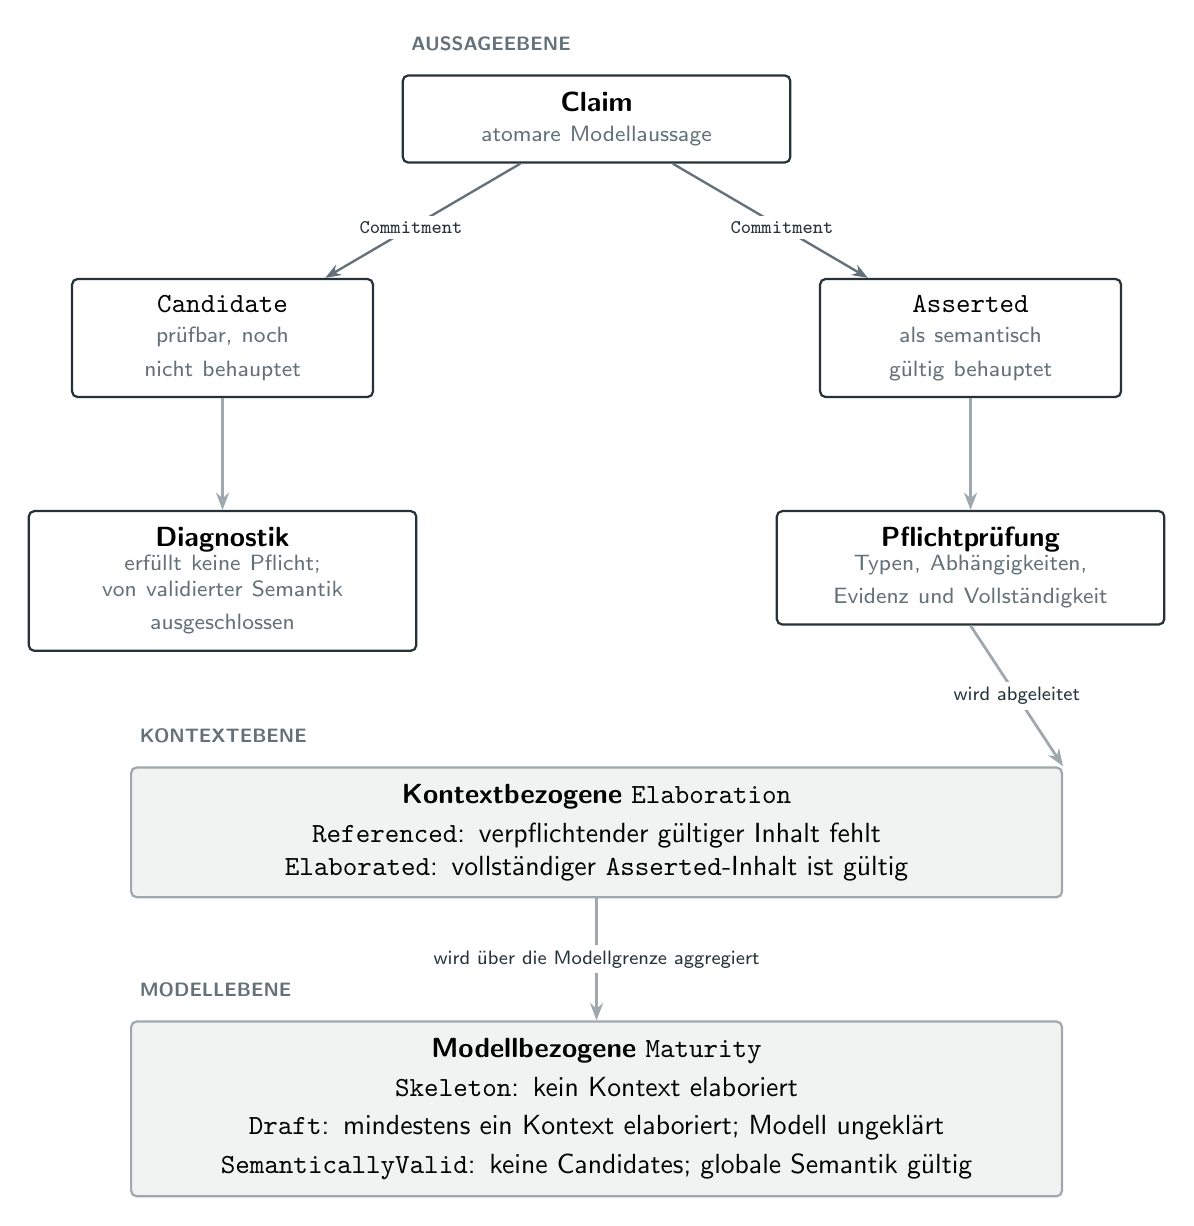
\begin{tikzpicture}[
  box/.style={
    draw=oink,
    fill=white,
    line width=0.8pt,
    rounded corners=2pt,
    minimum height=1.05cm,
    text width=4.5cm,
    align=center,
    inner sep=6pt,
    font=\sffamily
  },
  state/.style={box, text width=3.4cm},
  derived/.style={box, draw=oaccent, fill=osoft, text width=11.4cm},
  flow/.style={-{Stealth[length=2.2mm]}, draw=oaccent, line width=1pt},
  branch/.style={-{Stealth[length=2mm]}, draw=omuted, line width=0.85pt},
  relation/.style={
    fill=white,
    align=center,
    inner xsep=4pt,
    inner ysep=2pt,
    text=oink,
    font=\sffamily\scriptsize
  },
  level/.style={font=\sffamily\scriptsize\bfseries, text=omuted}
]

\node[box] (claim) {
  \textbf{Claim}\\[-1pt]
  {\footnotesize\color{omuted}atomare Modellaussage}
};
\node[level, anchor=south west] at ([yshift=0.18cm]claim.north west) {
  AUSSAGEEBENE
};

\node[state, below left=1.45cm and 0.35cm of claim] (candidate) {
  \textbf{\texttt{Candidate}}\\[-1pt]
  {\footnotesize\color{omuted}prüfbar, noch nicht behauptet}
};
\node[state, below right=1.45cm and 0.35cm of claim] (asserted) {
  \textbf{\texttt{Asserted}}\\[-1pt]
  {\footnotesize\color{omuted}als semantisch gültig behauptet}
};

\draw[branch] (claim) -- node[relation, pos=0.56] {\texttt{Commitment}} (candidate);
\draw[branch] (claim) -- node[relation, pos=0.56] {\texttt{Commitment}} (asserted);

\node[box, below=1.42cm of candidate] (excluded) {
  \textbf{Diagnostik}\\[-1pt]
  {\footnotesize\color{omuted}erfüllt keine Pflicht;\\
  \mbox{von validierter Semantik}\\
  ausgeschlossen}
};
\node[box, below=1.42cm of asserted] (validation) {
  \textbf{Pflichtprüfung}\\[-1pt]
  {\footnotesize\color{omuted}Typen, Abhängigkeiten,\\
  Evidenz und Vollständigkeit}
};

\draw[flow] (candidate) -- (excluded);
\draw[flow] (asserted) -- (validation);

\node[derived, below=1.62cm of $(excluded.south)!0.5!(validation.south)$] (elaboration) {
  \textbf{Kontextbezogene \texttt{Elaboration}}\\[2pt]
  \texttt{Referenced}: verpflichtender gültiger Inhalt fehlt
  \qquad
  \texttt{Elaborated}: vollständiger \texttt{Asserted}-Inhalt ist gültig
};
\node[level, anchor=south west] at ([yshift=0.18cm]elaboration.north west) {
  KONTEXTEBENE
};

\draw[flow] (validation.south) -- node[relation] {wird abgeleitet} (elaboration.north east);

\node[derived, below=1.55cm of elaboration] (maturity) {
  \textbf{Modellbezogene \texttt{Maturity}}\\[2pt]
  \texttt{Skeleton}: kein Kontext elaboriert
  \\[2pt]
  \texttt{Draft}: mindestens ein Kontext elaboriert; Modell ungeklärt
  \\[2pt]
  \texttt{SemanticallyValid}: keine Candidates; globale Semantik gültig
};
\node[level, anchor=south west] at ([yshift=0.18cm]maturity.north west) {
  MODELLEBENE
};

\draw[flow] (elaboration) -- node[relation] {wird über die Modellgrenze aggregiert} (maturity);

\end{tikzpicture}
\end{document}
